\documentclass[11pt,a4paper]{article}
\usepackage[T1]{fontenc}
\usepackage[utf8]{inputenc}
\usepackage{mathpazo}
\usepackage{xcolor}
\usepackage[protrusion=true,expansion=false]{microtype}
\usepackage[margin=2.4cm]{geometry}
\usepackage{amsmath,amssymb,booktabs,graphicx,caption}
\usepackage[colorlinks=true,linkcolor=blue!50!black,citecolor=blue!50!black,urlcolor=blue!50!black]{hyperref}
\captionsetup{font=small,labelfont=bf}
\setlength{\parskip}{0.4em}\setlength{\parindent}{0pt}
\newcommand{\RV}{\mathrm{RV}}
\newcommand{\E}{\mathbb{E}}

\title{\textbf{Forecasting Bitcoin Realized Volatility}\\[0.3em]
\large Econometric models versus machine learning in a rolling out-of-sample study}
\author{Ayoub Guenbib\\ \small École Polytechnique (X2025), applied mathematics}
\date{September 2026}

\begin{document}
\maketitle

\begin{abstract}
\sloppy\noindent We forecast next-day realized variance of BTC/\allowbreak USDT, computed from 5-minute Binance returns over 2019--2026.
Naive, GARCH(1,1) and HAR benchmarks are compared with XGBoost and an LSTM on 1{,}338 out-of-sample days,
using a rolling 1{,}000-day window, the QLIKE loss and Diebold--Mariano tests. HAR models built on intraday
data dominate GARCH, and a weekend dummy lowers QLIKE by a further 15\%. Machine-learning models reduce QLIKE by about
16\% relative to HAR+weekend, but a linear HAR fed with the same inputs is statistically indistinguishable
from XGBoost ($p=0.73$): the gain comes from feature engineering, chiefly intraweek seasonality, rather than from non-linearity.
\end{abstract}

\section{Data and realized variance}

We use Binance spot klines for BTC/\allowbreak USDT at a 5-minute frequency, from January 2019 to August 2026.
Let $P_{t,i}$ be the close of the $i$-th 5-minute bar of day $t$ (UTC) and $r_{t,i}=\log P_{t,i}-\log P_{t,i-1}$, with $M=288$ bars per day.
The daily return and the daily realized variance are
\begin{equation}
r_t=\sum_{i=1}^{M} r_{t,i}, \qquad \RV_t=\sum_{i=1}^{M} r_{t,i}^2 .
\end{equation}
Under a continuous semimartingale model $d\log P_s=\mu_s\,ds+\sigma_s\,dW_s$, $\RV_t$ converges to the integrated variance
$\int_{t-1}^{t}\sigma_s^2\,ds$ as $M\to\infty$ (Andersen et al., 2003), so it is a far more precise proxy of daily variance than
$r_t^2$. Days with fewer than $90\%$ of the bars are dropped, which leaves about 2{,}790 days.

\paragraph{Stylized facts.}
(i) $\RV_t$ is extremely skewed (skewness $\approx 21$, excess kurtosis $\approx 615$), whereas $y_t=\log\RV_t$ is close to Gaussian
(skewness $0.13$, excess kurtosis $0.85$); all models therefore target $y_{t+1}$.
(ii) Returns are nearly unpredictable (first-order autocorrelation $-0.07$).
(iii) $y_t$ has long memory: its autocorrelation is $0.70$ at lag 1 and still $0.27$ at lag 30.
(iv) The autocorrelation of $y_t$ peaks every 7 days: although Bitcoin trades continuously, volatility is markedly lower on weekends,
when traditional markets and institutional desks are closed.

\section{Models}

\paragraph{Naive.} $\widehat{\RV}_{t+1}=\RV_t$.

\paragraph{GARCH(1,1).} On daily returns (Bollerslev, 1986),
\begin{equation}
r_t=\mu+\varepsilon_t,\quad \varepsilon_t=\sigma_t z_t,\quad \sigma_t^2=\omega+\alpha\,\varepsilon_{t-1}^2+\beta\,\sigma_{t-1}^2,
\end{equation}
with $z_t$ standardized Student-$t$, estimated by maximum likelihood; the forecast is $\sigma^2_{t+1\mid t}$.

\paragraph{HAR family.} The heterogeneous autoregressive model (Corsi, 2009) approximates long memory with averages over three horizons.
With $y^{(w)}_t=\frac17\sum_{j=0}^{6}y_{t-j}$ (7 days, since crypto trades every day) and $y^{(m)}_t=\frac1{30}\sum_{j=0}^{29}y_{t-j}$,
\begin{equation}
y_{t+1}=\beta_0+\beta_d\,y_t+\beta_w\,y^{(w)}_t+\beta_m\,y^{(m)}_t+\gamma^{\top}D_{t+1}+\varepsilon_{t+1},
\end{equation}
estimated by OLS. \emph{HAR} has no calendar term; \emph{HAR+weekend} uses a single dummy $D_{t+1}$, equal to one when day $t+1$ is a Saturday or a Sunday;
\emph{HAR+dow} uses six weekday dummies (Monday as reference); \emph{HAR-X} additionally includes $y_{t-1},\dots,y_{t-6}$, the vol-of-vol
(7-day standard deviation of $y$), $r_t$, $|r_t|$ and $\min(r_t,0)$ (leverage effect), i.e.\ exactly the inputs given to the ML models.

\paragraph{Machine learning.} \emph{XGBoost} (Chen \& Guestrin, 2016): gradient-boosted trees of depth 3, learning rate $0.03$,
subsampling $0.8$, up to 1{,}000 trees with early stopping. \emph{LSTM} (Hochreiter \& Schmidhuber, 1997): one layer of 32 units on standardized
30-day sequences of the same features, Adam with weight decay $10^{-4}$, early stopping (patience 20).
\emph{Ensemble}: equal-weight average of the HAR+weekend, XGBoost and LSTM variance forecasts.

\paragraph{From log to variance.} Every model except Naive and GARCH predicts $\hat\mu_{t+1}=\widehat{\E}[y_{t+1}\mid\mathcal F_t]$.
If $y_{t+1}\mid\mathcal F_t\sim\mathcal N(\mu,s^2)$ then $\E[\RV_{t+1}\mid\mathcal F_t]=e^{\mu+s^2/2}$, so we report
$\widehat{\RV}_{t+1}=\exp(\hat\mu_{t+1}+\hat s^2/2)$, with $\hat s^2$ the residual variance (in-window for linear models,
on the validation block for ML models). Omitting this correction biases forecasts downwards, which QLIKE penalizes heavily.

\section{Forecasting protocol}

The out-of-sample period runs from 1 January 2023 to 30 August 2026 (1{,}338 days). All models use a rolling window of the last 1{,}000
days, so that every forecast of $\RV_{t+1}$ uses only information available at the end of day $t$. HAR models are refit every day, GARCH every
20 days and ML models every 60 days; for the latter, the last 200 days of each window serve for early stopping and for $\hat s^2$.

\paragraph{Loss functions.} Besides MSE and MSE on logs, the main criterion is
\begin{equation}
\mathrm{QLIKE}(\RV,h)=\frac{\RV}{h}-\log\frac{\RV}{h}-1\;\ge 0,
\end{equation}
which is zero iff $h=\RV$. Up to constants it is the negative Gaussian log-likelihood of a return with variance $h$. It depends only on the
ratio $\RV/h$, so crisis days do not dominate the average as they do under MSE, and it penalizes under-prediction more than over-prediction
(a forecast of half the true variance costs $0.31$, twice the true variance $0.19$). Crucially, QLIKE and MSE are the only standard losses that
rank forecasts consistently when the target is a noisy but unbiased proxy of the true variance (Patton, 2011).

\paragraph{Diebold--Mariano test.} For two models with losses $L^{(1)}_t,L^{(2)}_t$, let $d_t=L^{(1)}_t-L^{(2)}_t$ and $\bar d$ its mean over $n$ days. Then
\begin{equation}
\mathrm{DM}=\frac{\bar d}{\sqrt{\widehat{\Omega}/n}},\qquad
\widehat{\Omega}=\hat\gamma_0+2\sum_{h=1}^{5}\Bigl(1-\tfrac{h}{6}\Bigr)\hat\gamma_h ,
\end{equation}
where $\hat\gamma_h$ are sample autocovariances of $d_t$ (Newey--West). Under the null of equal predictive accuracy, $\mathrm{DM}$ is asymptotically
$\mathcal N(0,1)$ (Diebold \& Mariano, 1995); with rolling-window estimation this remains valid for comparing nested models (Giacomini \& White, 2006).
A negative statistic means that model 1 is more accurate.

\section{Results}

\begin{table}[h]
\centering\small
\begin{tabular}{lccc}
\toprule
& Estimate & Std.\ error & $t$ \\
\midrule
Constant & $-0.511$ & 0.131 & $-3.9$ \\
$y_t$ (daily) & $0.340$ & 0.019 & $18.2$ \\
$y^{(w)}_t$ (weekly) & $0.479$ & 0.032 & $15.1$ \\
$y^{(m)}_t$ (monthly) & $0.088$ & 0.030 & $2.9$ \\
Weekend dummy & $-0.619$ & 0.029 & $-21.4$ \\
\bottomrule
\end{tabular}
\caption{HAR+weekend estimated on the full sample (interpretation only), $R^2=0.62$.}
\label{tab:har}
\end{table}

Table~\ref{tab:har} confirms the stylized facts. The persistence $\beta_d+\beta_w+\beta_m=0.91$ is high, with the weekly component dominating.
The weekend coefficient implies $e^{-0.62}\approx0.54$: variance is about $46\%$ lower on weekends, i.e.\ volatility about $27\%$ lower, and it is the most
significant regressor.

\begin{table}[h]
\centering\small
\begin{tabular}{lccccc}
\toprule
Model & QLIKE & vs Naive & MSE log & DM vs HAR+weekend & DM vs XGBoost \\
\midrule
Naive        & 0.5433 & ---       & 0.7916 & $+8.71$ ($<$0.001) & --- \\
GARCH(1,1)   & 0.4159 & $-23\%$   & 1.0444 & $+4.16$ ($<$0.001) & --- \\
HAR          & 0.3466 & $-36\%$   & 0.6597 & $+5.58$ ($<$0.001) & --- \\
HAR+weekend  & 0.2943 & $-46\%$   & 0.4751 & ---                & $+1.40$ (0.161) \\
HAR+dow      & 0.2688 & $-51\%$   & 0.3969 & $-3.83$ ($<$0.001) & $+0.57$ (0.567) \\
HAR-X        & 0.2586 & $-52\%$   & \textbf{0.3777} & $-4.67$ ($<$0.001) & $+0.35$ (0.728) \\
XGBoost      & \textbf{0.2477} & $\mathbf{-54\%}$ & 0.4578 & $-1.40$ (0.161) & --- \\
LSTM         & 0.2606 & $-52\%$   & 0.4286 & $-1.16$ (0.245)    & $+0.70$ (0.483) \\
Ensemble     & 0.2485 & $-54\%$   & 0.4342 & $-1.90$ (0.057)    & $+0.07$ (0.941) \\
\bottomrule
\end{tabular}
\caption{Out-of-sample results, 2023-01-01 to 2026-08-30 (1{,}338 days). DM: Diebold--Mariano statistic on QLIKE, $p$-value in parentheses.}
\label{tab:oos}
\end{table}

\begin{figure}[h]
\centering
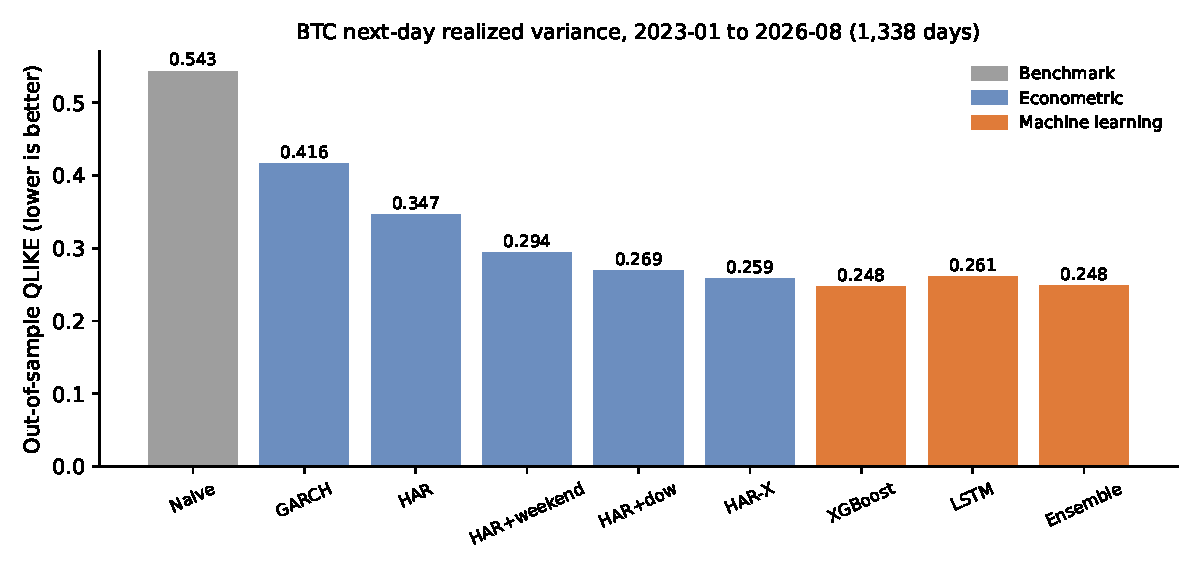
\includegraphics[width=0.82\textwidth]{qlike_comparison.pdf}
\caption{Out-of-sample QLIKE by model.}
\end{figure}

Three conclusions emerge from Table~\ref{tab:oos}.

\textbf{1. Intraday information beats daily returns.} Every HAR variant dominates GARCH. GARCH only sees daily returns, a very noisy signal,
so its forecasts are smooth and miss both spikes and the weekly cycle; its MSE on logs is even worse than the naive forecast.

\textbf{2. Calendar effects are the largest single gain.} The weekend dummy cuts QLIKE by $15\%$ relative to HAR, and weekday dummies by a further $9\%$,
both highly significant.

\textbf{3. The ML advantage is a feature effect, not a non-linearity effect.} XGBoost reaches the lowest QLIKE ($-16\%$ vs HAR+weekend) and the ensemble
the lowest MSE, but neither is significantly better than HAR+weekend at the $5\%$ level. XGBoost's most important features by gain are the weekend
indicator, the next day of the week, the weekly average and $y_{t-6}$ (same weekday one week earlier), i.e.\ calendar information. Once the linear model receives
the same inputs (HAR-X), it significantly beats HAR+weekend, obtains the best MSE on logs, and is statistically indistinguishable from XGBoost ($p=0.73$),
while remaining interpretable and essentially free to estimate.

\section{Limitations and extensions}

The study covers a single asset and a one-day horizon, with fixed ML hyperparameters. Five-minute sampling limits but does not remove microstructure noise;
realized kernels or subsampling would be more robust, and jump-robust measures (bipower variation) would allow HAR-J or HARQ specifications (Bollerslev et al., 2016).
Pairwise DM tests could be replaced by a Model Confidence Set (Hansen et al., 2011). Natural extensions are multi-horizon forecasts (1, 5 and 22 days),
other crypto-assets, and an economic evaluation, for instance volatility targeting or Value-at-Risk backtests driven by each forecast.

\section*{References}
\small
\begin{itemize}\setlength{\itemsep}{0pt}
\item Andersen, T., Bollerslev, T., Diebold, F. X. \& Labys, P. (2003). Modeling and forecasting realized volatility. \emph{Econometrica}, 71(2).
\item Bollerslev, T. (1986). Generalized autoregressive conditional heteroskedasticity. \emph{Journal of Econometrics}, 31(3).
\item Bollerslev, T., Patton, A. J. \& Quaedvlieg, R. (2016). Exploiting the errors: a simple approach for improved volatility forecasting. \emph{Journal of Econometrics}, 192(1).
\item Chen, T. \& Guestrin, C. (2016). XGBoost: a scalable tree boosting system. \emph{Proceedings of KDD}.
\item Corsi, F. (2009). A simple approximate long-memory model of realized volatility. \emph{Journal of Financial Econometrics}, 7(2).
\item Diebold, F. X. \& Mariano, R. S. (1995). Comparing predictive accuracy. \emph{Journal of Business \& Economic Statistics}, 13(3).
\item Giacomini, R. \& White, H. (2006). Tests of conditional predictive ability. \emph{Econometrica}, 74(6).
\item Hansen, P. R., Lunde, A. \& Nason, J. M. (2011). The model confidence set. \emph{Econometrica}, 79(2).
\item Hochreiter, S. \& Schmidhuber, J. (1997). Long short-term memory. \emph{Neural Computation}, 9(8).
\item Newey, W. K. \& West, K. D. (1987). A simple, positive semi-definite, heteroskedasticity and autocorrelation consistent covariance matrix. \emph{Econometrica}, 55(3).
\item Patton, A. J. (2011). Volatility forecast comparison using imperfect volatility proxies. \emph{Journal of Econometrics}, 160(1).
\end{itemize}
\end{document}
